% Split-fill plot marks used at force-vector endpoints.
\documentclass[border=2pt]{standalone}
\usepackage{tikz}
\usetikzlibrary{arrows.meta,plotmarks}

\begin{document}
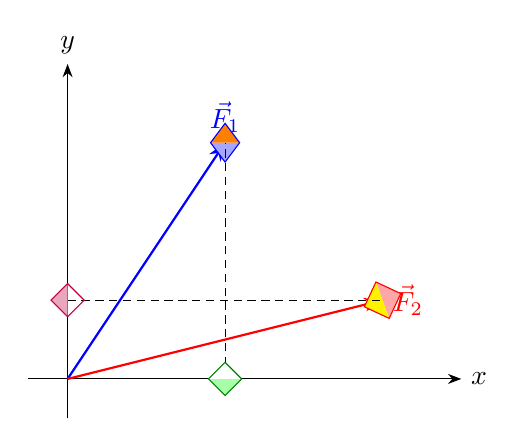
\begin{tikzpicture}[>=Stealth]
  \draw[->] (-0.5,0) -- (5,0) node[right] {$x$};
  \draw[->] (0,-0.5) -- (0,4) node[above] {$y$};
  \draw[thick,blue,-Stealth] (0,0) -- (2,3) node[above] {$\vec F_1$};
  \draw[thick,red,-Stealth] (0,0) -- (4,1) node[right] {$\vec F_2$};
  \draw[blue,fill=blue!35,mark color=orange,mark size=7pt]
    plot[mark=halfdiamond*] coordinates {(2,3)};
  \draw[red,fill=red!35,mark color=yellow,mark size=7pt]
    plot[mark=halfsquare right*,mark options={rotate=20}] coordinates {(4,1)};
  \draw[densely dashed] (2,0) -- (2,3);
  \draw[densely dashed] (0,1) -- (4,1);
  \draw[green!50!black,fill=green!35,mark color=white,mark size=6pt]
    plot[mark=halfsquare*] coordinates {(2,0)};
  \draw[purple,fill=purple!35,mark color=none,mark size=6pt]
    plot[mark=halfsquare left*] coordinates {(0,1)};
\end{tikzpicture}
\end{document}
